\let\negmedspace\undefined
\let\negthickspace\undefined
\documentclass[journal,12pt,twocolumn]{IEEEtran}
\usepackage{gensymb}
\usepackage{amssymb}
\usepackage[cmex10]{amsmath}
\usepackage{amsthm}
\usepackage[export]{adjustbox}
\usepackage{bm}
\usepackage{longtable}
\usepackage{enumitem}
\usepackage{mathtools}
 \usepackage{tikz}
\usepackage[breaklinks=true]{hyperref}
\usepackage{listings}
\usepackage{color}                                            %%
\usepackage{array}                                            %%
\usepackage{longtable}                                        %%
\usepackage{calc}                                             %%
\usepackage{multirow}                                         %%
\usepackage{hhline}                                           %%
\usepackage{ifthen}                                           %%
\usepackage{lscape}     
\usepackage{multicol}
% \usepackage{enumerate}
\DeclareMathOperator*{\Res}{Res}
\renewcommand\thesection{\arabic{section}}
\renewcommand\thesubsection{\thesection.\arabic{subsection}}
\renewcommand\thesubsubsection{\thesubsection.\arabic{subsubsection}}
\renewcommand\thesectiondis{\arabic{section}}
\renewcommand\thesubsectiondis{\thesectiondis.\arabic{subsection}}
\renewcommand\thesubsubsectiondis{\thesubsectiondis.\arabic{subsubsection}}
\hyphenation{op-tical net-works semi-conduc-tor}
\def\inputGnumericTable{}                                 %%
\lstset{
frame=single, 
breaklines=true,
columns=fullflexible
}
\begin{document}

\raggedbottom
\setlength{\parindent}{0pt}
\vspace{3cm}
\title{AI1110-Assignment 1}
\author{Vedant Bhandare\\CS21BTECH11007}
\maketitle
\newpage
\bigskip
\renewcommand{\thefigure}{\theenumi}
\renewcommand{\thetable}{\theenumi}

\section{\underline{\textbf{Question}}}
The circumference of the base of a cylindrical vessel is 132 cm and its height is 25 cm. Find the

\begin{enumerate}
    \item radius of the cylinder
    \item volume of cylinder.(use $\pi = \frac{22}{7}$)
\end{enumerate}
\section{\underline{\textbf{Solution}}}
Let $r$ and $h$ be the radius of the base and height of the cylindrical vessel, respectively.
Let $C_{base}$ be its base circumference and $V$ be its volume.\\

We know that,
\begin{align}
    C_{base} = 2\pi{r}\\
    V = \pi{r^2h}
\end{align}

\subsection{\underline{\textbf{Radius of the cylinder}}}
\begin{align}
C_{base} = 2\pi{r}\\
132 = 2\pi{r}\\
132 = 2\times\frac{22}{7}\times{r}\\
r = 21
\end{align}
\begin{center}
    Thus the radius of base of the cylindrical vessel is $21 cm$.
\end{center}
\subsection{\underline{\textbf{Volume of the cylinder}}}
\begin{align}
V = \pi{r^2h}\\
V = \frac{22}{7}\times21^2\times25\\
V = 34650
\end{align}
\begin{center}
    {Thus, the volume of the cylindrical vessel is $34650 \hspace{1mm} cm^3.$}
\end{center}
\begin{figure}
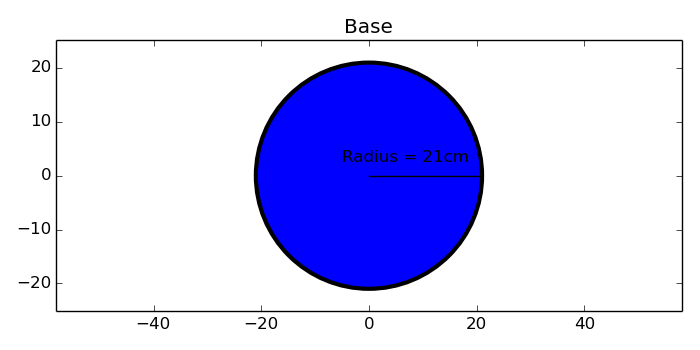
\includegraphics[width = \columnwidth]{Figures/Base.png}
\caption{Base of the cylindrical vessel with radius 21 cm}
\label{fig:fig1}

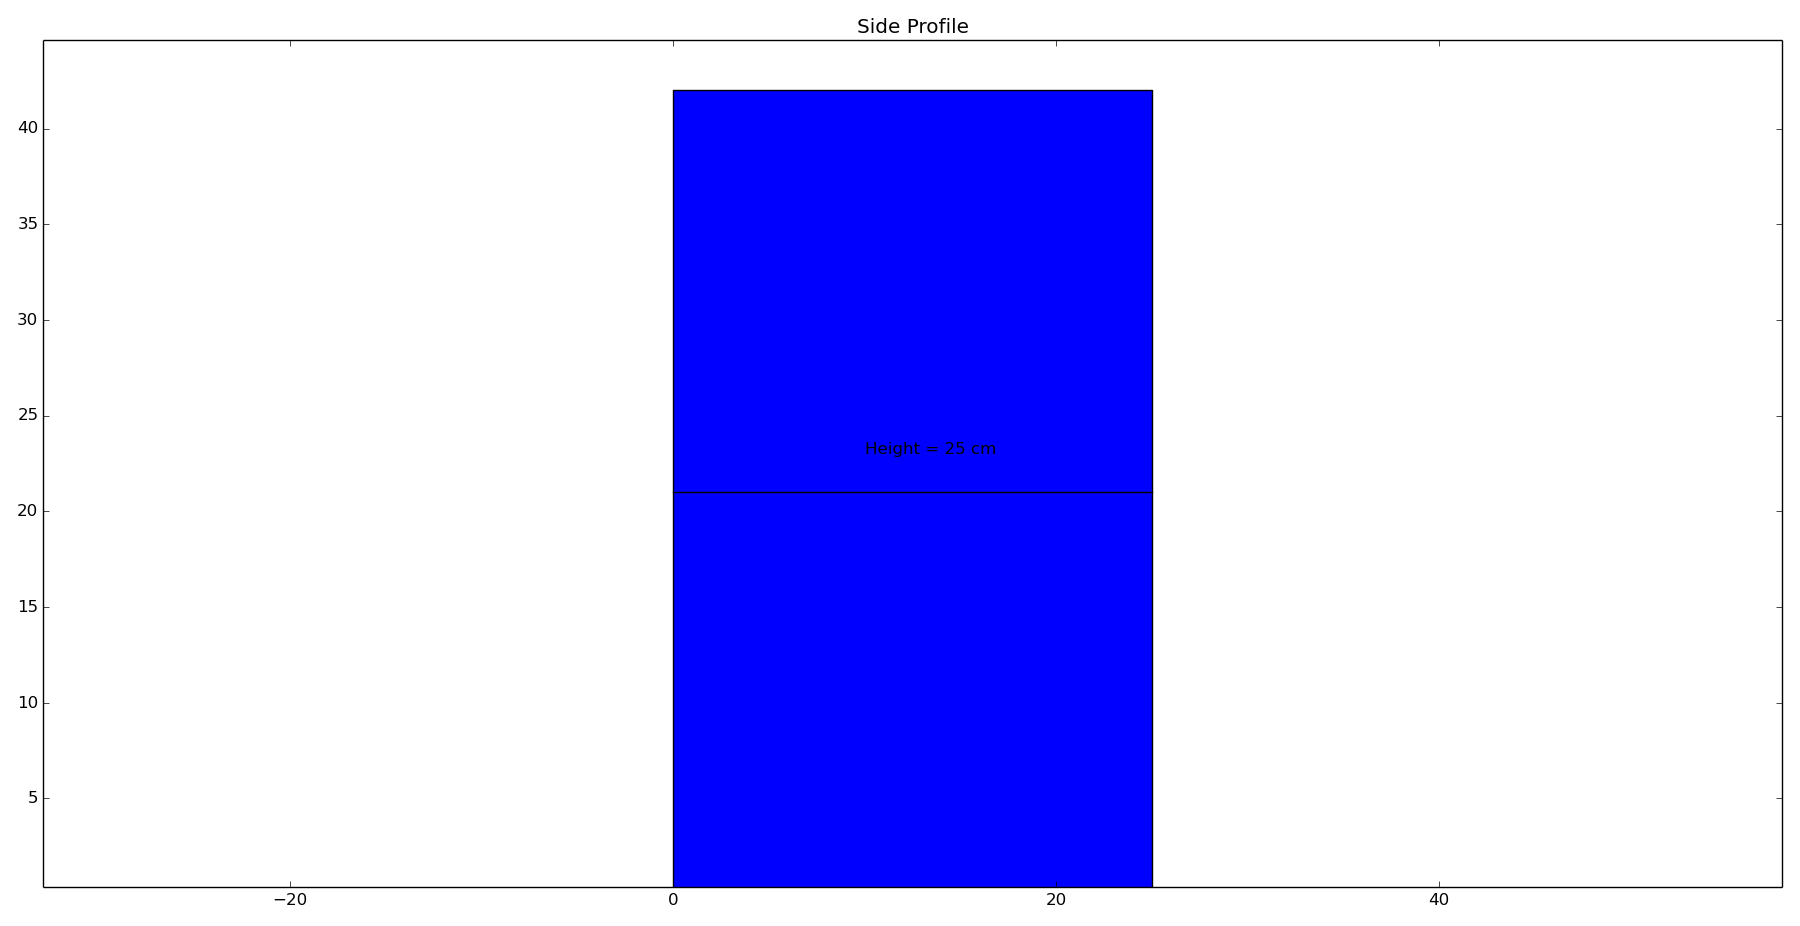
\includegraphics[width = \columnwidth]{Figures/Side Profile.png}
\caption{Side view of the cylindrical vessel with height 25 cm}
\label{fig:fig2}
\end{figure}
\begin{center}
\begin{tabular}{|c|c|c|c|c|}
\hline
 & & & Formula & Value Derived \\
 \hline
\multirow{4}{*}{\rotatebox[origin = c]{90}{Variables}} & \multirow{2}{*}{Given} & $C_{base}$ & $2 \pi r$ & 132 cm \\
\cline{3-5}
 & & $h$ & $\frac{V}{\pi r^2}$ & 25 cm \\
\cline{2-5}
 & \multirow{2}{*}{Unknown} & $r$ & $\frac{C_{base}}{2\pi}$ & 21 cm \\
\cline{3-5}
 & & $V$ & $\pi r^2h$ & 34650 cm^3\\
\hline
\end{tabular}
\end{center}
\begin{center}
\caption{TABLE 1: Variables, Formulae and their Values Derived}
\end{center}
\end{document}